\chapter{Практическая часть}
\label{ch:chap2}

\section*{\textbf{Введение}}

На практике продолжаем реализовывать сигналы разной формы. На этом занятии реализую сигнал параболической формы и треугольный сигнал.

\section*{\textbf{Треугольный сигнал}}

Я буду формировать такой сигнал по следующему принципу:

\begin{enumerate}
    \item Если бит равен единице, то в момент длительности сигнала $\frac{\tau}{2}$ буду
    задавать максимальное значение, а в остлаьных случаях буду задавать нули. Таким образом в одной точке будет образовываться пик,
    который и будет придавать сигналу форму треугольного.
    \item Если бит равен 0, то на всей длительности $\tau$ сигнал будет принимать 0.
\end{enumerate}

\subsection*{\textbf{Программная реализация}}

\begin{lstlisting}
    #define TAU 10
    #define TAU_ON_ELEMENT 20

    int16_t* bits_to_triangle_signal(uint8_t* bits, int bits_count, int tx_mtu){

    // allocate memory
    int16_t* tx_buff = (int16_t*)malloc(sizeof(int16_t) * tx_mtu * 2);

    // iterate on bitts
    for (int i = 0; i < bits_count; ++i)
    {   
        // fill tx_buff with samples
        for(int j = i*TAU_ON_ELEMENT; j < i*TAU_ON_ELEMENT + 20 && j < tx_mtu*2; j+=2){
            if(bits[i] && j == i*TAU_ON_ELEMENT + 8){
                tx_buff[j] = 2047 << 4;    // I
                tx_buff[j+1] = -2047 << 4; // Q
            } else{
                tx_buff[j] = 0;      //I
                tx_buff[j+1] = 0;    //Q
            }
        }
    }

    return tx_buff;
}
\end{lstlisting}

Код полностью идентичен коду, который использовался для создания прямоугольного сигнала. Единственное отличие заключается в условии

\begin{lstlisting}
    j == i*TAU_ON_ELEMENT + 8
\end{lstlisting}

Это условие как раз и позволяет выбрать одну конкретную точку, в которой задается максимальное значение.

Визуализируем сигнал:



Отправим сформированный сигнал и посмотрим на результат после приема.

\begin{figure}[H]
    \centering
    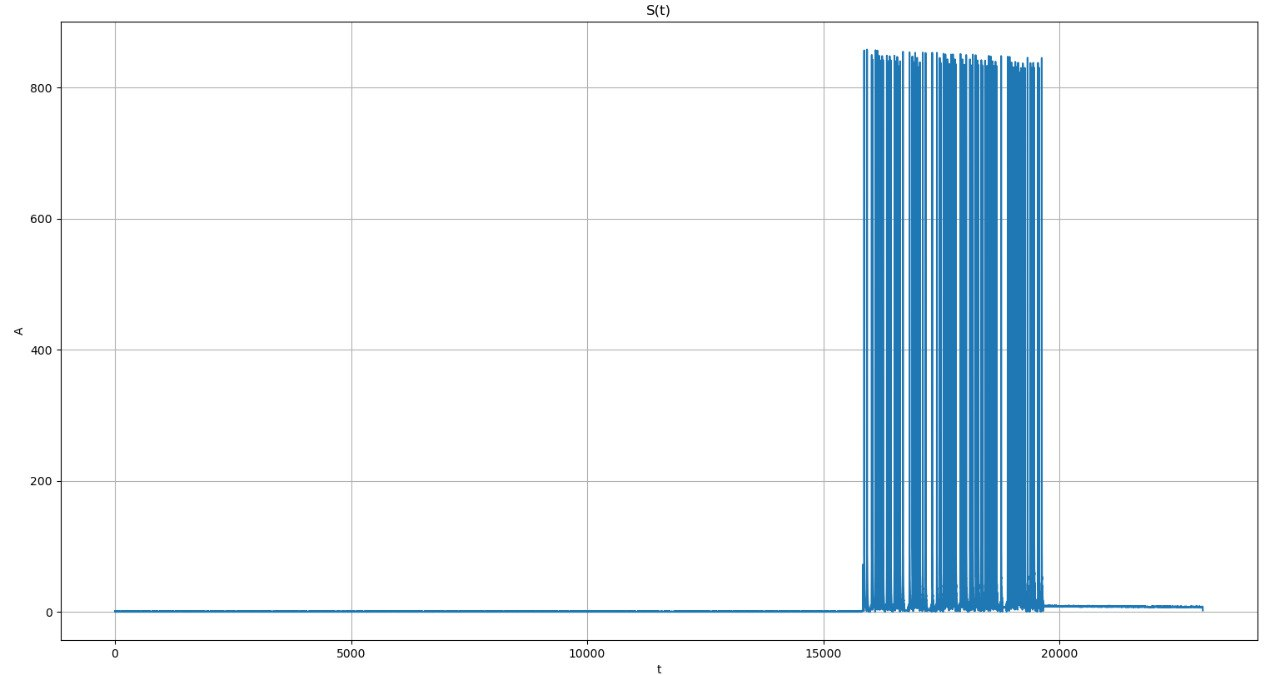
\includegraphics[width=1.0\textwidth]{triangle.png}
    \caption{Пример принятого треугольного сигнала}
\end{figure}

\section*{\textbf{Параболический сигнал}}

Сформируем параболу, перебирая точки от $-\frac{tx\_mtu}{10}$ до $-\frac{tx\_mtu}{10} + 2\frac{tx\_mtu}{10}$, где $tx\_mtu$ - кол-во семплов,
передаваемых за раз. Деление на 10 используется для масштабирования, чтобы не возводить большие числа в квадрат.

\subsection*{\textbf{Программная реализация}}

\begin{lstlisting}
    int16_t* parabola_signal(int tx_mtu){

    // allocate memory
    int16_t* tx_buff = (int16_t*)malloc(sizeof(int16_t) * tx_mtu * 2);

    float coef = -tx_mtu / 10;

    for (int i = 0; i < 2 * tx_mtu; i+=2)
    {
        tx_buff[i] = int16_t(coef * coef);   // I
        tx_buff[i+1] = int16_t(coef * coef); // Q

        coef += 0.1;
    }

    return tx_buff;
}
\end{lstlisting}

\subsection*{\textbf{Визуализация}}

\begin{figure}[H]
    \centering
    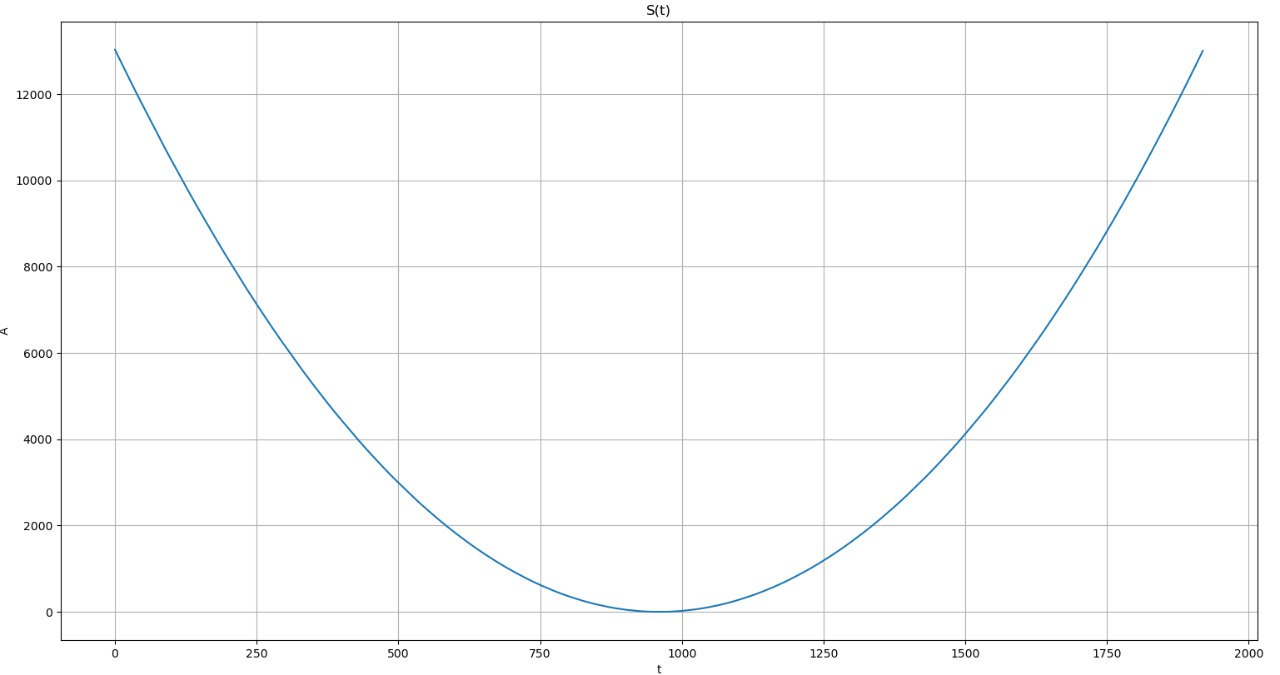
\includegraphics[width=1.0\textwidth]{parab.png}
    \caption{Пример сигнала в виде параболы}
\end{figure}

\subsection*{\textbf{Визуализация после приема}}

\begin{figure}[H]
    \centering
    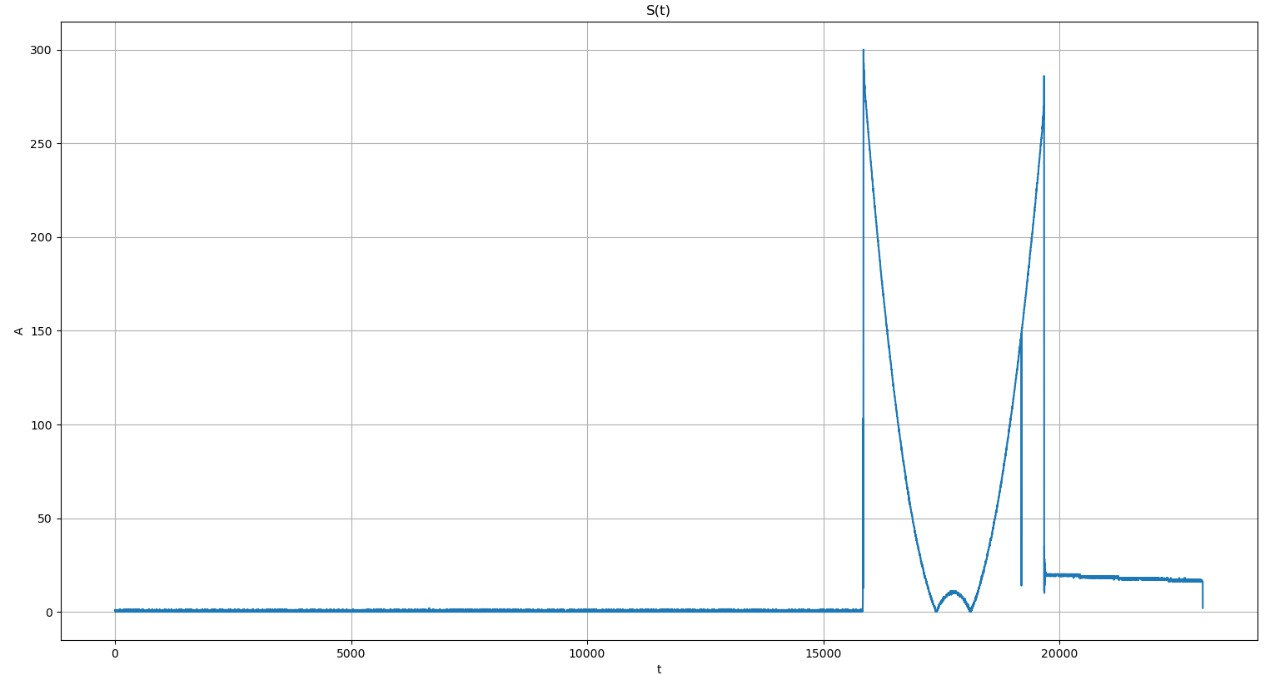
\includegraphics[width=1.0\textwidth]{rx_parab.png}
    \caption{Пример сигнала в виде параболы на приеме}
\end{figure}

Можем наблюдать параболу в нашем сигнале, по центру парабола отображена вверх, потому что я строил график модуля сигнала.

\section*{\textbf{Реализация BPSK модуляции}}

Шаги по реализации:

\begin{enumerate}
    \item Написать BPSK модуляцию (логика маппера)
    \item На основе I и Q, полученных на прошлом шаге, сгенерировать прямоугольные импульсы (логика формирующего фильтра)
    \item Перемножить прямоугольные импульсы на несущее колебание
    \item Проанализировать полученные результаты и сделать вывод
\end{enumerate}

\subsection*{\textbf{BPSK модулятор}}

Реализация на языке С:

\begin{lstlisting}
double* BPSK_modulation(int* bits, int bits_count){
    //allocate memory
    double* IQ_samples = (double*)malloc(sizeof(double) * bits_count * 2);
    //iterate on bits
    for(int i,j = 0; i < bits_count * 2; i+=2){
        if(bits[j]){
            IQ_samples[i] = 1;      // I
            IQ_samples[i + 1] = 0;  // Q
        }else{
            IQ_samples[i] = -1;     // I
            IQ_samples[i + 1] = 0;  // Q
        }

        ++j;
    }

    return IQ_samples;
}
\end{lstlisting}

Сначала выделяем память под IQ семплы, т.к на каждый бит приходится 1 семпл, а на 1 семпл - 2 числа (I и Q), то размер массива 
с семплами должен быть вдвое больше кол-ва бит. Далее перебираем биты и в зависимости от его значения формируем семпл. В результирующем
массиве I и Q идут в строгой последовательности $I_0,Q_0,I_1,Q_1,...,I_N,Q_N$. Массив в дальнейшем запишется в файл.

\subsection*{\textbf{Формирующий фильтр}}

На языке Python парсим файл с семплами из прошлого шага. Далее формируем прямоугольные импульсы. Визуализация импульсов:

\begin{figure}[H]
    \centering
    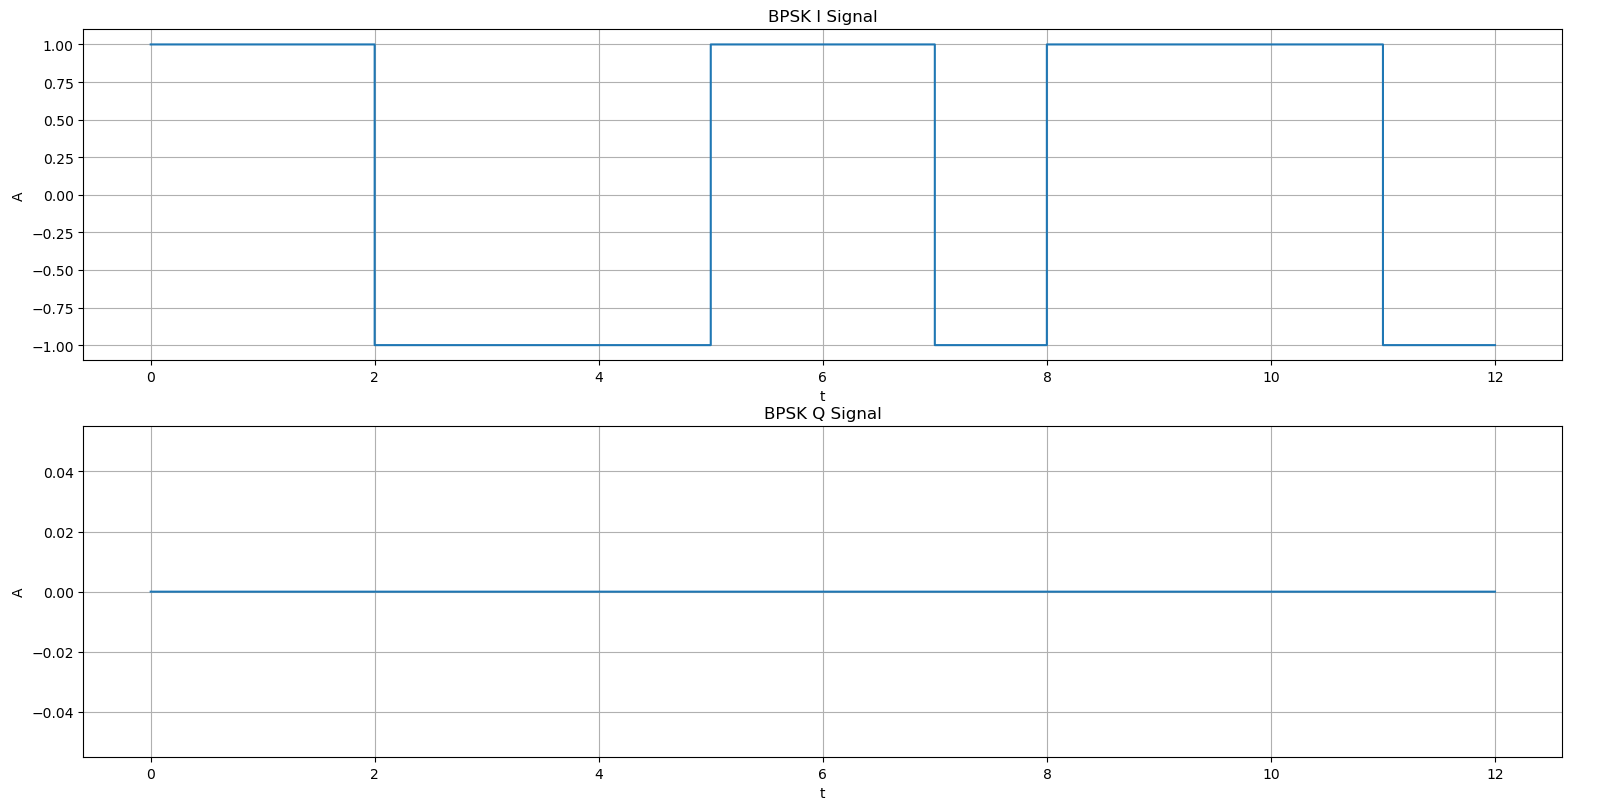
\includegraphics[width=1.0\textwidth]{bpsk_symb.png}
    \caption{Символы}
\end{figure}

Здесь явно видно, что в BPSK модуляции квадратурная составляющая всегда равна 0. Я передавал последовательность в 12 бит и это
заняло 12 секунд, т.е на каждый бит приходился 1 символ, который длился 1 секунду.

\subsection*{\textbf{Перемножение с несущим колебанием}}

Теперь перемножим символы с несущим колебанием. В роли несущего колебания я использовал $cos(2\pi f_сt)$ и $-sin(2\pi f_сt)$ с частотой
$f_с = 1$. В реальности частоты несущих колебаний в разы больше, но для наглядности я взял маленькое значение. Этот процесс можно
сравнить с наложением маски, где маской является прямоугольный сигнал. Если посмотреть на схему цифровой системы связи, которая
была дана в разделе с теорией, то этот процесс происходит в цепи, которая следует после формирующего фильтра. Визуализация результата:

\begin{figure}[H]
    \centering
    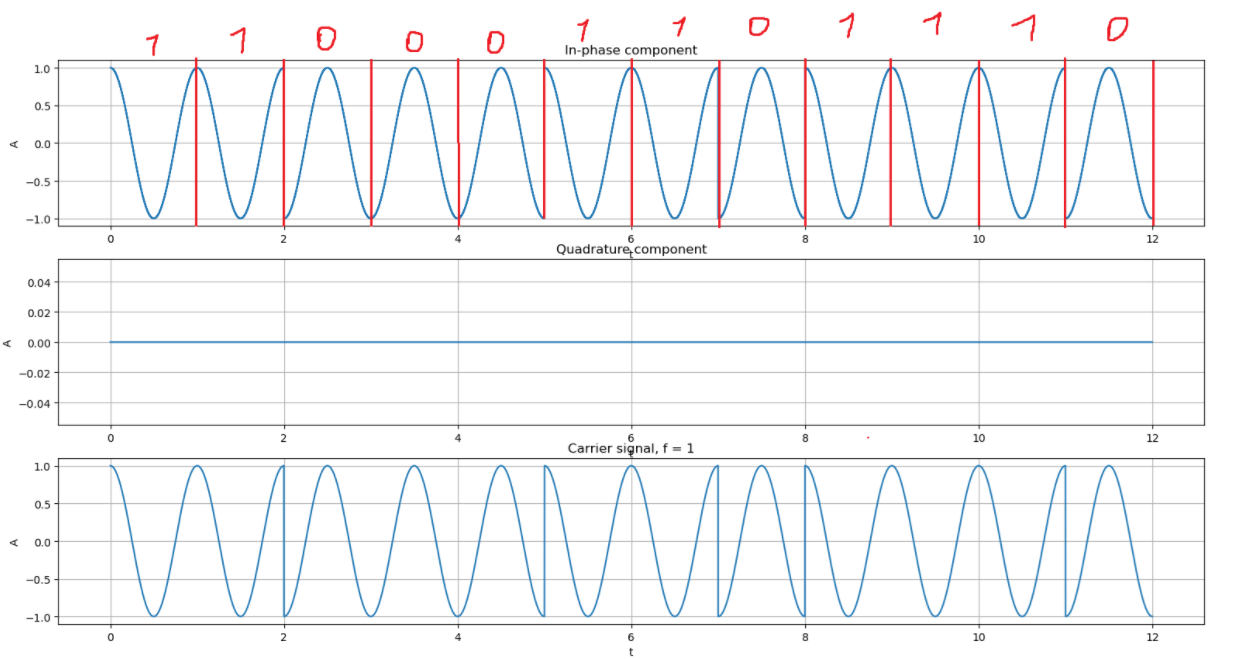
\includegraphics[width=1.0\textwidth]{bpsk_mul_symb.png}
    \caption{Перемножение с несущим сигналом}
\end{figure}

Можем видеть, что квадратурная компонента по прежнему равна 0, т.е в сигнале присутствует только $cos$. В синфазной компоненте
можем видеть, как меняется фаза колебания, которая отражает значение бита. Если фаза равна 0, то передается 1, если фаза равна $\pi$,
то передается 0. В местах, где меняется фаза, происходит смена значения бита. Таким образом можно восстановить передаваемую битовую
последовательность. Результирующий сигнал будет иметь вид синфазной компоненты, т.к квадратурная всегда равна 0.

\section*{\textbf{Реализация QPSK модуляции}}

Шаги по реализации будут в точности такие же, как у BPSK модуляции, но слегка будет отличаться реализация.\\

Реализация на языке С:

\begin{lstlisting}
double* QPSK_modulation(int* bits, int bits_count){
    //allocate memory
    double* IQ_samples = (double*)malloc(sizeof(double) * bits_count);
    //iterate on bits
    for(int i = 0; i < bits_count; i+=2){
        if(bits[i]){
            IQ_samples[i] = -1;          //I
            if(bits[i + 1]){
                IQ_samples[i + 1] = -1;  //Q
            }else{
                IQ_samples[i + 1] = 1; // Q
            }
        }else{
            IQ_samples[i] = 1;         //I
            if(bits[i + 1]){
                IQ_samples[i + 1] = 1;  //Q
            }else{
                IQ_samples[i + 1] = -1; //Q
            }
        }
    }


    return IQ_samples;
}
\end{lstlisting}

Заметим, что в случае QPSK модуляции массив под семплы вдвое меньше, т.к в QPSK модуляции на 1 семпл приходится 2 бита.

\subsection*{\textbf{Формирующий фильтр}}

Визуализация импульсов:

\begin{figure}[H]
    \centering
    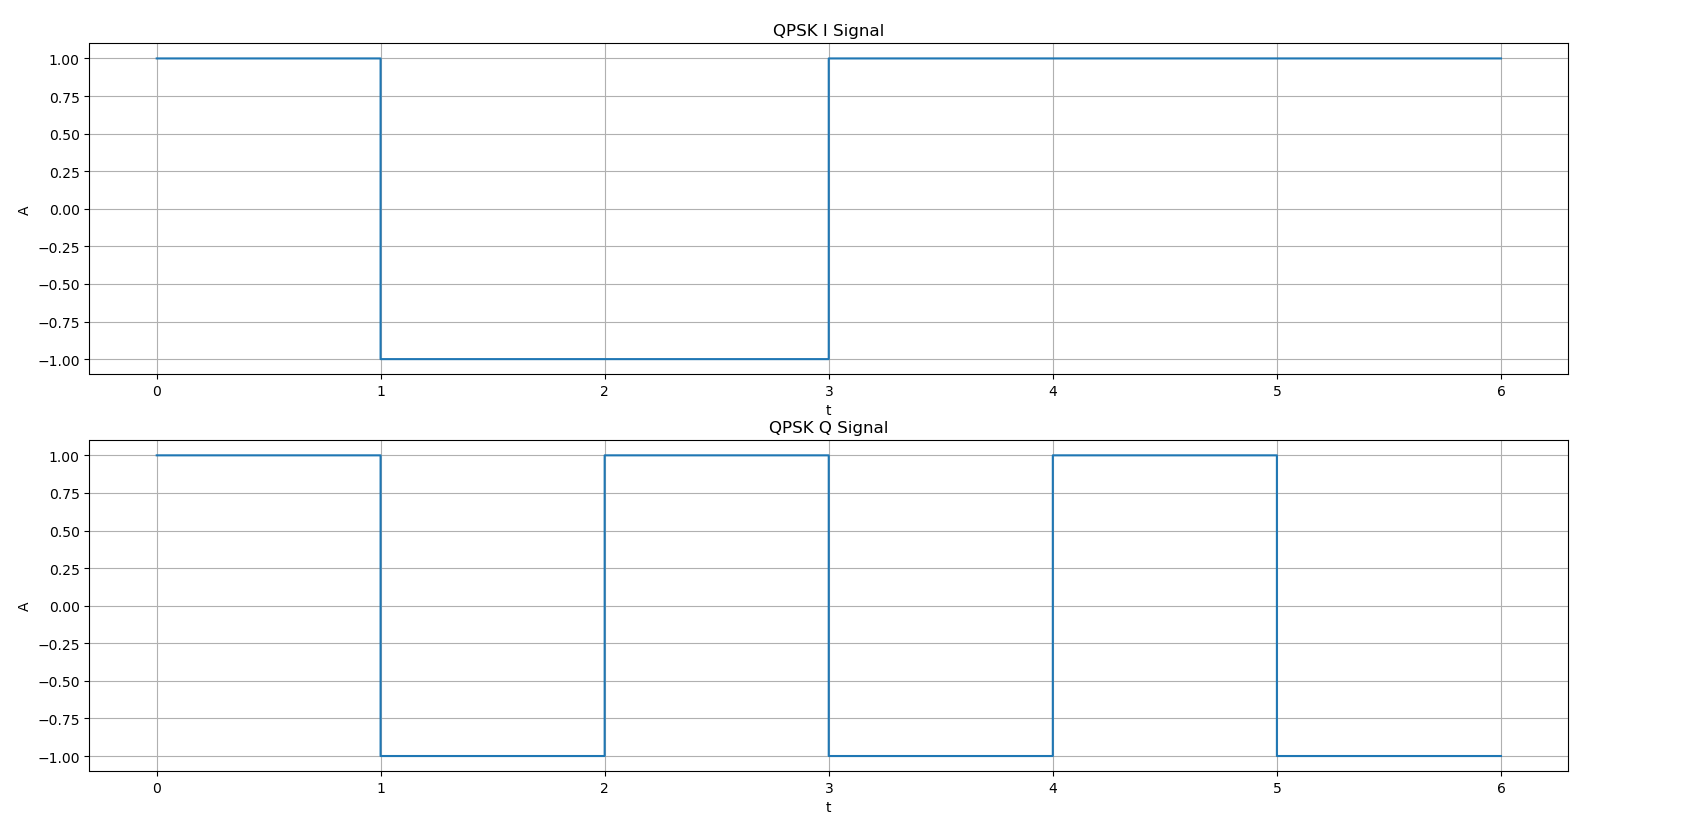
\includegraphics[width=1.0\textwidth]{qpsk_symb.png}
    \caption{Символы}
\end{figure}

Можем заметить, что появляется квадратурная часть. Также можно заметить, что та же последовательность из 12 бит передается уже
за 6 секунд. Это связано с тем, что в QPSK на семпл приходится 2 бита. Можно сделать вывод о том, что чем больше точек в сигнальном
созвездии, тем выше скорость передачи данных. 1 символ длится уже не 1 секунду, а 0.5 секунд (на графике чуть неверный масштаб)

\subsection*{\textbf{Перемножение с несущим колебанием}}

Визуализация результата:

\begin{figure}[H]
    \centering
    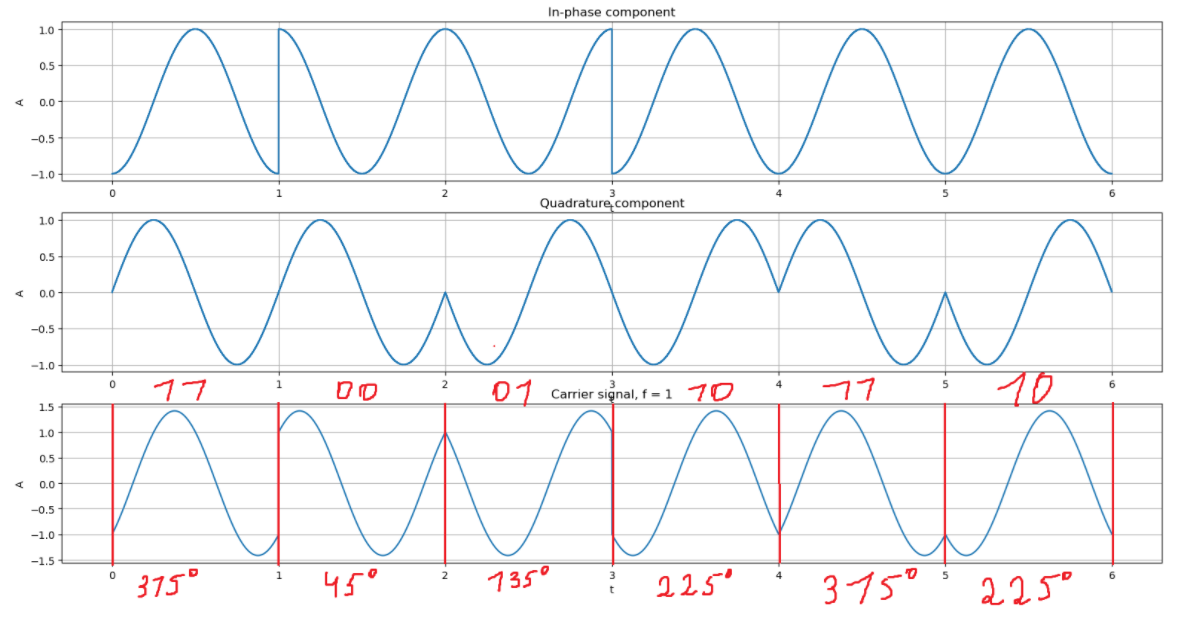
\includegraphics[width=1.0\textwidth]{qpsk_mul_symb.png}
    \caption{Перемножение с несущим сигналом}
\end{figure}

Можем видеть, что квадратурная компонента теперь не равна 0, т.е в сигнале присутствует $cos$ и $sin$. Еще можно заметить, что
максимальная амплитуда в результирующем сигнале уже не равна 1, а равна $\sqrt{I^2+Q^2} = \sqrt{1^2+1^2} = \sqrt{2}$.
Результирующий сигнал будет иметь вид $Icos(2\pi f_ct) - Qsin(2\pi f_ct)$. 

\endinput
